% !TEX program = xelatex
\documentclass{ctexart}
\usepackage{xeCJK}
\setCJKmainfont{楷体-简 黑体}
\usepackage{geometry}
\geometry{left=2.5cm,right=2.5cm}
\usepackage[colorlinks,linkcolor=blue]{hyperref}
\CTEXsetup[format={\Large\bfseries}]{section}
\usepackage{listings}
\usepackage{xcolor}
\title{
    \LARGE
    Web信息处理与应用 Lab2-1: \\
    网络中节点影响力及社区发现: Erdös共同作者网络的挖掘
}
\author{
    张劲暾\quad PB16111485 \qquad
    冉礼豪\quad PB16050176 \qquad
    胡煜霄\quad PB16050193 
}
\begin{document}
    \maketitle
    \tableofcontents
    \section{数据集描述}
    \paragraph{
        文件Erdos.html给出了Paul Erdos的511名共同作者名单,与他们下面列出的共同作者一起。
        给出了与鄂尔多斯的第一份联合文件的日期,其次是联合出版物的数量(如果它不止一个)。 名称后面有一个星号表明这个Erdos合作者是众所周知的死者。
    }
    \section{数据预处理与Erdös共同作者网络的建立}
    \paragraph{
        数据预处理策略:\\
        1. 由于这个图非常的大,所以可以忽略重名,死亡,合作数量等稀疏的信息以降低分析的复杂度。\\
        2. 利用networkx包建立网络结构。 \\
        3. 删除一些度数很少的节点降低分析时的干扰。\\
        4. 手动删除html标签和其他信息方便处理。\\
        共同作者网络初步建立如下图所示:(可以粗略地看到8个左右的社区)
    }
    \begin{center}
        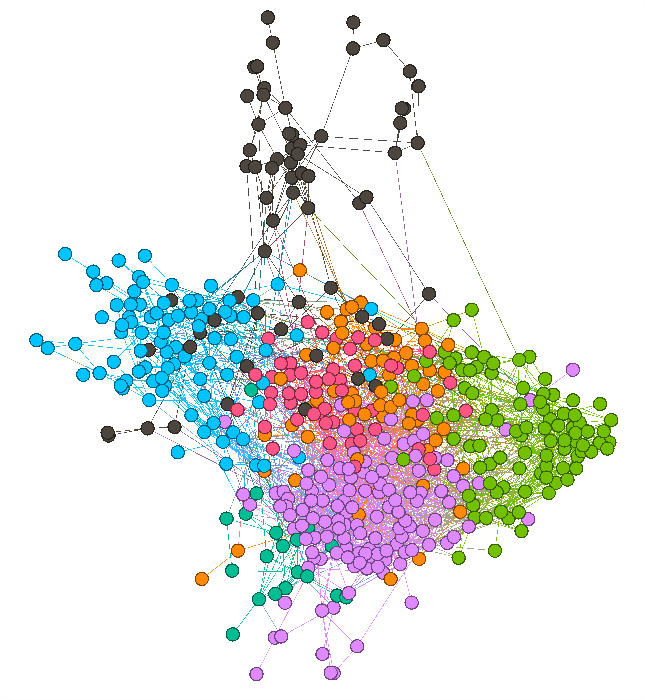
\includegraphics[height= 15cm] {b7.png}
    \end{center}
    \section{影响力分析}
    \subsection{Degree Centrality}
    \paragraph{
        Degree Centrality认为,度数越大的节点,越具有影响力,选取度数最大的50个节点,代码如下:\\
    }
    \begin{lstlisting}[language=python, basicstyle=\tiny,keywordstyle=\color{blue!100},commentstyle=\color{red!100!},frame=shadowbox, rulesepcolor=\color{red!20!green!20!blue!20}]
        # Degree Centrality Influence Analyse
        CoAuthGraphDict = nx.convert.to_dict_of_lists(CoAuthGraph)
        DegreeDict = {}
        for node in CoAuthGraph.nodes:
            DegreeDict[node] = len(CoAuthGraphDict[node])

        SortedDegree = sorted(DegreeDict.items(),key = lambda x:x[1],reverse = True)
        InfluentialAnalyseData = open("../data2/InfluentialAnalyseData.txt",'w')
        print("Top 50 of the most influential node under Degree Centrality: \n",end = '')
        InfluentialAnalyseData.write("Top 50 of the most influential node under Degree Centrality: \n")
        for i in range(50):
            print( str(i + 1) + ' : ' + str(SortedDegree[i]) + '\n',end = '')
        InfluentialAnalyseData.write( str(i + 1) + ' : ' + str(SortedDegree[i]) + '\n')
    \end{lstlisting}
    \subsection{Closeness Centrality}
    \paragraph{
        Closeness Centrality认为,到图上其他点平均距离越小的点,越具有影响力,选取到图上其他点平均距离最小的50个节点,代码如下:\\
    }
    \begin{lstlisting}[language=python, basicstyle=\tiny,keywordstyle=\color{blue!100},commentstyle=\color{red!100!},frame=shadowbox, rulesepcolor=\color{red!20!green!20!blue!20}]
        # Closeness Centrality Influence Analyse
        NumberOfNodes = len((list)(CoAuthGraph.nodes))
        ClosenessDict = {}
        for node_form in CoAuthGraph.nodes:
            SumDistanse = 0
            for node_to in CoAuthGraph.nodes:
                try:
                    SumDistanse += nx.shortest_path_length(CoAuthGraph,node_form,node_to)
                except nx.exception.NetworkXNoPath:
                    SumDistanse += NumberOfNodes * 10
            #print(node_form + str(( NumberOfNodes - 1 ) / SumDistanse))
            ClosenessDict[node_form] = ( NumberOfNodes - 1 ) / SumDistanse
        SortedCloseness = sorted(ClosenessDict.items(),key = lambda x:x[1],reverse = True)

        print("Top 50 of the most influential node under Closeness Centrality: \n",end = '')
        InfluentialAnalyseData.write("Top 50 of the most influential node under Closeness Centrality: \n")
        for i in range(50):
            print( str(i + 1) + ' : ' + str(SortedCloseness[i]) + '\n',end = '')
            InfluentialAnalyseData.write( str(i + 1) + ' : ' + str(SortedCloseness[i]) + '\n')
    \end{lstlisting}
    \subsection{两种方法的结果对比}
    \paragraph{
        Closeness Centrality 和 Degree Centrality 的运行结果对比如下:仔细观察会发现左右两行有很多相同的名字,所以两种方法都有一定的效果但并不完全相同
    }
    \begin{center}
        \scriptsize
        \begin{tabular}{|c|c|c|c|}
            \hline 
            Node & Degree Centrality & Node & Closeness Centrality \\
            \hline
            ALON,NOGAM. & 435 & ALON,NOGAM. & 0.0022076341214382735 \\
            \hline
            HARARY,FRANK' & 315 & GRAHAM,RONALDLEWIS & 0.0022072631603754877 \\
            \hline
            COLBOURN,CHARLESJOSEPH & 244 & FUREDI,ZOLTAN & 0.0022069908350490835 \\
            \hline
            SHELAH,SAHARON & 223 & BOLLOBAS,BELA & 0.002206952782513424\\
            \hline
            TUZA,ZSOLT & 223 & RODL,VOJTECH & 0.0022068420148237716\\
            \hline
            SALAMON,PETER & 220 & SPENCER,JOELHAROLD & 0.002206832714226083\\
            \hline
            WEST,DOUGLASBRENT & 201 & HARARY,FRANK & 0.0022066940600661356\\
            \hline
            GRAHAM,RONALDLEWIS & 196 & TUZA,ZSOLT & 0.0022066712345272027\\
            \hline
            LUCA,FLORIAN & 193 & CHUNG,FANRONGKING(GRAHAM) & 0.002206440046886851\\
            \hline
            HSU,DERBIAUFRANK & 170 & LOVASZ,LASZLO & 0.002206410887718393\\
            \hline
            BOLLOBAS,BELA & 166 & NESETRIL,JAROSLAV & 0.002206401590754258\\
            \hline
            PACH,JANOS & 154 & KLEITMAN,DANIELJ. & 0.0022063944067901788\\
            \hline
            KLEITMAN,DANIELJ. & 152 & WORMALD,NICHOLASCHARLES & 0.0022063145411641413\\
            \hline
            ODLYZKO,ANDREWMICHAEL & 151 & ODLYZKO,ANDREWMICHAEL & 0.0022063090479738155\\
            \hline
            JANSON,SVANTE & 149 & SOS,VERATURAN & 0.002206283272599896\\
            \hline
            RODL,VOJTECH & 145 & SZEMEREDI,ENDRE & 0.002206276089406274\\
            \hline
            LOVASZ,LASZLO & 145 & FRANKL,PETER & 0.0022062482021566843\\
            \hline
            CAMERON,PETERJ. & 145 & PACH,JANOS & 0.002206232146181265\\
            \hline
            CHUNG,FANRONGKING(GRAHAM) & 142 & BABAI,LASZLO & 0.0022060213275537617\\
            \hline
            SAKS,MICHAELEZRA & 140 & GYARFAS,ANDRAS & 0.00220593853205897\\
            \hline
            FABER,VANCE & 138 & RUZSA,IMREZ. & 0.0022058768619027257\\
            \hline
            LINIAL,NATHAN & 137 & TROTTER,WILLIAMTHOMAS & 0.0022058688365880113\\
            \hline
            HELL,PAVOL & 136 & SAKS,MICHAELEZRA & 0.0022058675694383943\\
            \hline
            DIACONIS,PERSIW. & 133 & FAUDREE,RALPHJASPER,JR. & 0.0022058667246727917\\
            \hline
            KOREN,ISRAEL & 132 & LUCZAK,TOMASZ & 0.0022058460281176437\\
            \hline
            HEDETNIEMI,STEPHENTRAVIS & 126 & STRAUS,ERNSTGABOR & 0.002205816884647457\\
            \hline
            SHALLIT,JEFFREYOUTLAW & 126 & CHVATAL,VACLAV(VASEK) & 0.002205783518431504\\
            \hline
            FUREDI,ZOLTAN & 123 & SIMONOVITS,MIKLOS & 0.0022057645128103795\\
            \hline
            WORMALD,NICHOLASCHARLES & 123 & WEST,DOUGLASBRENT & 0.0022057442405088376\\
            \hline
            NESETRIL,JAROSLAV & 122 & POMERANCE,CARLBERNARD & 0.0022056897605448053\\
            \hline
            KOSTOCHKA,ALEXANDRV. & 121 & WINKLER,PETERMANN & 0.002205646685269152\\
            \hline
            ARONOV,BORIS & 119 & KOSTOCHKA,ALEXANDRV. & 0.0022056357055660137\\
            \hline
            WINKLER,PETERMANN & 118 & HAJNAL,ANDRAS & 0.002205633594097173\\
            \hline
            HENNING,MICHAELANTHONY & 115 & COLBOURN,CHARLESJOSEPH & 0.0022055111358210045\\
            \hline
            SPENCER,JOELHAROLD & 114 & HELL,PAVOL & 0.002205485379086944\\
            \hline
            GODDARD,WAYNEDEAN & 114 & THOMASSEN,CARSTEN & 0.002205430489693633\\
            \hline
            CHARTRAND,GARYTHEODORE & 112 & KOMLOS,JANOS & 0.002205408534701299\\
            \hline
            POMERANCE,CARLBERNARD & 112 & JANSON,SVANTE & 0.0022053937575487355\\
            \hline
            MCKAY,BRENDANDAMIEN & 111 & BURR,STEFANANDRUS & 0.0022052814576604147\\
            \hline
            STINSON,DOUGLASROBERT & 111 & CHARTRAND,GARYTHEODORE & 0.002205266260057938\\
            \hline
            BABAI,LASZLO & 107 & FRAENKEL,AVIEZRISIEGMUND & 0.002205216447162765\\
            \hline
            HOFFMAN,ALANJEROME & 105 & LEHEL,JENO & 0.0022051839433512746\\
            \hline
            LUCZAK,TOMASZ & 105 & MCKAY,BRENDANDAMIEN & 0.002205110074615795\\
            \hline
            MCELIECE,ROBERTJAMES & 102 & ROTHSCHILD,BRUCELEE & 0.0022051024769694084\\
            \hline
            TETALI,PRASADVENKATASITARAMAVARA & 97 & CAMERON,PETERJ. & 0.0022050910805979933\\
            \hline
            CHUI,CHARLESKAM-TAI & 95 & LINIAL,NATHAN & 0.0022050505611202883\\
            \hline
            KLAWE,MARIAMARGARET & 93 & Seymour,PaulD. & 0.0022050497169803377\\
            \hline
            AVIS,DAVIDMICHAEL & 91 & SCHELP,RICHARDHERBERT & 0.0022049817658343815\\
            \hline
            FRAENKEL,AVIEZRISIEGMUND & 91 & TETALI,PRASADVENKATASITARAMAVARA & 0.0022049724809098574\\
            \hline
            TOVEY,CRAIGAARON & 91 & GRANVILLE,ANDREWJAMES & 0.0022049281675745407\\
            \hline
        \end{tabular}
    \end{center}
    \section{社区发现}
    \subsection{GirvanNewman算法的步骤}
    \paragraph{GirvanNewman算法的基本思想:在模块性没有达到要求之前,不断切除边界数最大的边。\\}
    \begin{lstlisting}[language=python, basicstyle=\small,keywordstyle=\color{blue!100},commentstyle=\color{red!100!},frame=shadowbox, rulesepcolor=\color{red!20!green!20!blue!20}]
        def run(self):
        while True:
            ModulQ = self.get_modularity()
            print("Get Modularity:" + str(ModulQ))
            if (ModulQ > self.Q) or (self.Graph.number_of_edges() == 0):
                break
            self.cut_bridge()
            #############################################################
            DegreeDict = (dict)(nx.degree(self.Graph))
            NodeList = list( self.Graph.nodes() )
            for node in NodeList:
                if DegreeDict[node] <= 1:
                    self.Graph.remove_node(node)
            #############################################################
    \end{lstlisting}
    \begin{lstlisting}[language=python, basicstyle=\small,keywordstyle=\color{blue!100},commentstyle=\color{red!100!},frame=shadowbox, rulesepcolor=\color{red!20!green!20!blue!20}]
        def get_modularity(self):
        print("Computing Modularity...")
        Communities = nx.connected_components(self.Graph)
        DegreeDict = (dict)(nx.degree(self.Graph))
        Modularity = 0.0
        Nodes = list(self.Graph.nodes())
        AdjMatrix = nx.adj_matrix(self.Graph)
        NumberOfEdges = nx.number_of_edges(self.Graph)
        
        for Com in Communities:
            for node_from in Com:
                for node_to in Com:
                    Modularity += ( 
                float(AdjMatrix[Nodes.index(node_from),Nodes.index(node_to)]) - 
                float(DegreeDict[node_from] * DegreeDict[node_to]) / 
                float(2 * NumberOfEdges) )

        Modularity = Modularity / ( 2 * NumberOfEdges )
        return Modularity
    \end{lstlisting}
    \begin{lstlisting}[language=python, basicstyle=\footnotesize,keywordstyle=\color{blue!100},commentstyle=\color{red!100!},frame=shadowbox, rulesepcolor=\color{red!20!green!20!blue!20}]
        def cut_bridge(self):
        OriginCommunityNum = nx.number_connected_components(self.Graph)
        NewCommunityNum = OriginCommunityNum
        print("Begin Cut ...",end ='\t')
        CutTimes = 0
        while NewCommunityNum <= OriginCommunityNum:

            # print("Computing Betweenness...",end='\t')
            EdgeBetweenness = nx.edge_betweenness_centrality(self.Graph)
            # print("Betweenness get.")
            CutTimes = CutTimes + 1
            ################################################################################
            # 这里每次只删除一条界边数最高的边
            # EBSortedOrder = sorted(EdgeBetweenness.items(),key=lambda x:x[1],reverse=True)
            # self.Graph.remove_edge(EBSortedOrder[0][0][0],EBSortedOrder[0][0][1])
            #################################################################################

            # 一次性删除所有界边数最高的边加快收敛速度:
            MaxEB = max(EdgeBetweenness.values())
            for edge, bet in EdgeBetweenness.items():
                if float(bet) == MaxEB:
                    self.Graph.remove_edge(edge[0],edge[1])

            NewCommunityNum = nx.number_connected_components(self.Graph)

        print("Cut: " + str(CutTimes) + " Edges.")
    \end{lstlisting}
    \paragraph{GirvanNewman算法的运行结果,可以看到一共有12个明显的社区,其中8个已经被划分出来了,此时的模块性已经大于0.5}
    \begin{center}
        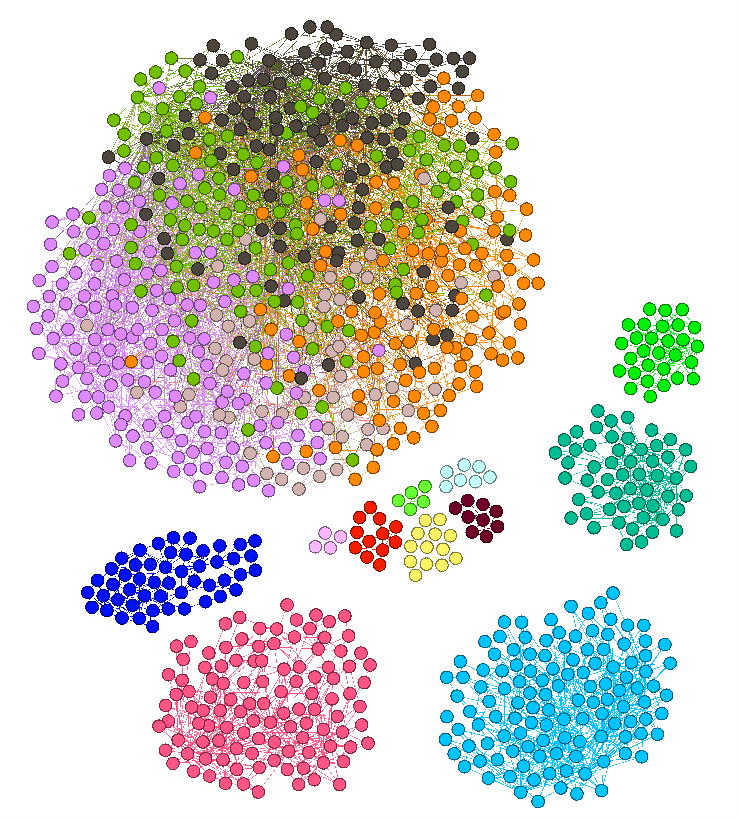
\includegraphics[height= 16cm] {GNCut2.png}
    \end{center}
    \subsection{NormalizedCut谱聚类算法的步骤}
    \paragraph{NormalizedCut谱聚类算法的核心思想是通过在图的Laplacian矩阵的特征向量组成的点的特征向量上运行聚类算法发现社区,代码如下:\\[50pt]}
    \begin{lstlisting}[language=python, basicstyle=\normalsize,keywordstyle=\color{blue!100},commentstyle=\color{red!100!},frame=shadowbox, rulesepcolor=\color{red!20!green!20!blue!20}]
        def run(self):
        EigenVectorForCut = self.spectral_cut()
        Clusters = self.k_means(EigenVectorForCut.T)
        Communities = self.get_community(Clusters)
        print(len(Communities))
        return Communitiesfootnotesize
    \end{lstlisting}
    \begin{lstlisting}[language=python, basicstyle=\normalsize,keywordstyle=\color{blue!100},commentstyle=\color{red!100!},frame=shadowbox, rulesepcolor=\color{red!20!green!20!blue!20}]
        def spectral_cut(self):
        '''
            Compute eigenvectors for Laplacian matrix of the graph
        '''
        DegreeDict = (dict)(nx.degree(self.Graph))
        self.D = np.diag(list(DegreeDict.values())).astype(float)
        self.D_05 = np.diag(list(DegreeDict.values())).astype(float)

        for i in range(self.D_05.shape[0]):
            if self.D_05[i][i] != 0:
                self.D_05[i][i] = self.D_05[i][i] ** (-0.5)
        self.M = nx.adjacency_matrix(self.Graph).todense()
        self.M.astype(float)
        LaplacianMatrix = 
        np.dot( np.dot( self.D_05, ( self.D - self.M ) ), self.D_05 )
        print("Getting eigenvectors...")
        EigenValues, EigenVectors = np.linalg.eig(LaplacianMatrix)
        print("Eigenvectors get.")
        return np.array( EigenVectors[:self.expected_community_number] )
    \end{lstlisting}
    \paragraph{
        NormalizedCut谱聚类算法的运行结果,这里在聚类时选择GirvanNewman算法的先验结果,即
        聚为12个类,删除掉一些边缘节点之后,可以看到NormalizedCut谱聚类算法同样可以找到相似的12个
        社区的核心结构,但是在一些边缘节点上划分错误较大,所以社区不是很”丰满“,在这一点上比GirvanNewman算法略差,
        但在运行速度上快于GirvanNewman算法。
    }
    \begin{center}
        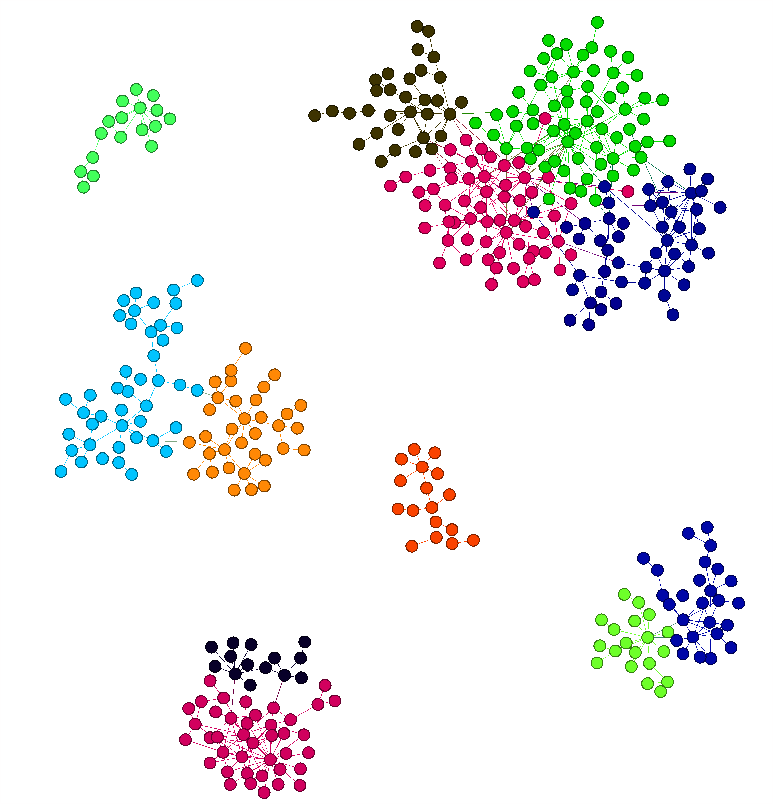
\includegraphics[height= 16cm] {NCCut.png}
    \end{center}
\end{document}